\documentclass{exam}

\usepackage{pdfpages}
\usepackage[utf8]{inputenc} %To allow typesetting öäü

\begin{document}

\null

\vspace{2cm}

\null

\cfoot{}

\begin{center}
\begin{Huge}
Aufgabensammlung
\end{Huge}
\end{center}

\vspace{5cm}

\begin{center}
\begin{Large}
PVK Informatik
\end{Large}
\end{center}

\vspace{5cm}

\begin{center}
\begin{Large}
GianAndrea Müller - 2018

\vspace{2cm}

basierend auf Prüfungen vom D-INFK
\end{Large}
\end{center}

\newcommand{\Lone}{L1: Datentypen, Literale, Operatoren, Präzedenz}
\newcommand{\Ltwo}{L2: Pointer, Referenzen, Dynamische Allokation}
\newcommand{\Lthree}{L3: Arrays, vector, struct}
\newcommand{\Lfour}{L4: Syntax, ASCII Code, string}
\newcommand{\Lfive}{L5: Verzweigungen, Schleifen}
\newcommand{\Lsix}{L6: Funktionen, Gültigkeitsbereich, Überladungen}
\newcommand{\Lseven}{L7: Stellenwertsysteme, EBNF}
\newcommand{\Leight}{L8: Klassen, Dynamische Datenstrukturen}
\newcommand{\Lnine}{L9: Vererbung}

\newpage                                                                                                                                                                                                                                                                                       
%Exercises for lecture 1

\lhead{PHYSExam\_IFMP\_2018\_01}\rhead{\Lone}

\includepdf[pages=3,pagecommand={\pagestyle{plain}}]{PruefungenPHYS/Exam_IFMP_2018_01.pdf}

\rhead{Lösung}

\includepdf[pages=3,pagecommand={\pagestyle{plain}}]{PruefungenPHYS/Exam_IFMP_2018_01_Solution.pdf}



\lhead{PHYSExam\_IFMP\_2017\_08}\rhead{\Lone}

\includepdf[pages=3,pagecommand={\pagestyle{plain}}]{PruefungenPHYS/Exam_IFMP_2017_08.pdf}

\rhead{Lösung}

\includepdf[pages=3,pagecommand={\pagestyle{plain}}]{PruefungenPHYS/Exam_IFMP_2017_08_Solution.pdf}



\lhead{PHYSExam\_IFMP\_2017\_01}\rhead{\Lone}

\includepdf[pages=3,pagecommand={\pagestyle{plain}}]{PruefungenPHYS/Exam_IFMP_2017_01.pdf}

\rhead{Lösung}

\includepdf[pages=3,pagecommand={\pagestyle{plain}}]{PruefungenPHYS/Exam_IFMP_2017_01_Solution.pdf}

\newpage
%Exercises for lecture 2

\lhead{PHYSExam\_Jan\_27\_2016}\rhead{\Ltwo}

\includepdf[scale=0.9,pages={16,17},pagecommand={\pagestyle{plain}}]{PruefungenPHYS/Exam_Jan_27_2016.pdf}

\rhead{Lösung}

\includepdf[scale=0.9,pages={17},pagecommand={\pagestyle{plain}}]{PruefungenPHYS/Exam_Jan_27_2016_solution.pdf}

\newpage

\lhead{ITETExam\_DITET\_InfI\_2017\_08}\rhead{\Ltwo}

\includepdf[scale=0.9,pages={12,13},pagecommand={\pagestyle{plain}}]{PruefungenITET/Exam_DITET_InfI_2017_08.pdf}

\rhead{Lösung}

\includepdf[scale=0.9,pages=12,pagecommand={\pagestyle{plain}}]{PruefungenITET/Exam_DITET_InfI_2017_08-Solution.pdf}

\newpage
%Exercises for lecture 3

\lhead{PHYSExam\_Jan\_21\_2015}\rhead{\Lthree}

\includepdf[scale=0.9,pages={4,5},pagecommand={\pagestyle{plain}}]{PruefungenPHYS/Exam_Jan_21_2015.pdf}

\rhead{Lösung}

\includepdf[scale=0.9,pages={5},pagecommand={\pagestyle{plain}}]{PruefungenPHYS/Exam_Jan_21_2015_solution.pdf}

\newpage

\lhead{ITETExam\_DITET\_InfI\_2017\_02}\rhead{\Lthree}

\includepdf[scale=0.9,pages={4,5},pagecommand={\pagestyle{plain}}]{PruefungenITET/Exam_DITET_InfI_2017_02.pdf}

\rhead{Lösung}

\includepdf[scale=0.9,pages=5,pagecommand={\pagestyle{plain}}]{PruefungenITET/Exam_DITET_InfI_2017_02-Solution.pdf}

\newpage

%Exercises for lecture 4

\lhead{PHYSExam\_Jan\_27\_2016}\rhead{\Lfour}

\includepdf[scale=0.9,pages={10,11},pagecommand={\pagestyle{plain}}]{PruefungenPHYS/Exam_Jan_27_2016.pdf}

\rhead{Lösung}

\includepdf[scale=0.9,pages={11},pagecommand={\pagestyle{plain}}]{PruefungenPHYS/Exam_Jan_27_2016_solution.pdf}

\newpage

\lhead{PHYSExam\_Jan\_21\_2015}\rhead{\Lfour}

\includepdf[scale=0.9,pages={8,9},pagecommand={\pagestyle{plain}}]{PruefungenPHYS/Exam_Jan_21_2015.pdf}

\rhead{Lösung}

\includepdf[scale=0.9,pages={9},pagecommand={\pagestyle{plain}}]{PruefungenPHYS/Exam_Jan_21_2015_solution.pdf}

\newpage

%Exercises for lecture 5

\lhead{PHYSExam\_IFMP\_2018\_01}\rhead{\Lfive}

\includepdf[scale=0.9,pages={4},pagecommand={\pagestyle{plain}}]{PruefungenPHYS/Exam_IFMP_2018_01.pdf}

\rhead{Lösung}

\includepdf[scale=0.9,pages={4},pagecommand={\pagestyle{plain}}]{PruefungenPHYS/Exam_IFMP_2018_01_solution.pdf}

\newpage

\lhead{PHYSExam\_IFMP\_2017\_08}\rhead{\Lfive}

\includepdf[scale=0.9,pages={4},pagecommand={\pagestyle{plain}}]{PruefungenPHYS/Exam_IFMP_2017_08.pdf}

\rhead{Lösung}

\includepdf[scale=0.9,pages={4},pagecommand={\pagestyle{plain}}]{PruefungenPHYS/Exam_IFMP_2017_08_solution.pdf}

\newpage

\lhead{PHYSExam\_IFMP\_2017\_01}\rhead{\Lfive}

\includepdf[scale=0.9,pages={4},pagecommand={\pagestyle{plain}}]{PruefungenPHYS/Exam_IFMP_2017_01.pdf}

\rhead{Lösung}

\includepdf[scale=0.9,pages={4},pagecommand={\pagestyle{plain}}]{PruefungenPHYS/Exam_IFMP_2017_01_solution.pdf}

\newpage

%Exercises for lecture 6

\lhead{ITETExam\_DITET\_InfI\_2017\_02}\rhead{\Lsix}

\includepdf[scale=0.9,pages={6,7},pagecommand={\pagestyle{plain}}]{PruefungenITET/Exam_DITET_InfI_2017_02.pdf}

\rhead{Lösung}

\includepdf[scale=0.9,pages={6,7},pagecommand={\pagestyle{plain}}]{PruefungenITET/Exam_DITET_InfI_2017_02-Solution.pdf}

\newpage

\lhead{PHYSExam\_Jan\_27\_2016}\rhead{\Lsix}

\includepdf[scale=0.9,pages={12,13},pagecommand={\pagestyle{plain}}]{PruefungenPHYS/Exam_Jan_27_2016.pdf}

\rhead{Lösung}

\includepdf[scale=0.9,pages={13},pagecommand={\pagestyle{plain}}]{PruefungenPHYS/Exam_Jan_27_2016_solution.pdf}

%Exercises for lecture 7

\newpage

\lhead{PHYSExam\_IFMP\_2018\_01}\rhead{\Lseven}

\includepdf[scale=0.9,pages={7},pagecommand={\pagestyle{plain}}]{PruefungenPHYS/Exam_IFMP_2018_01.pdf}

\rhead{Lösung}

\includepdf[scale=0.9,pages={7},pagecommand={\pagestyle{plain}}]{PruefungenPHYS/Exam_IFMP_2018_01_solution.pdf}

\newpage

\lhead{PHYSExam\_IFMP\_2017\_01}\rhead{\Lseven}

\includepdf[scale=0.9,pages={7},pagecommand={\pagestyle{plain}}]{PruefungenPHYS/Exam_IFMP_2017_01.pdf}

\rhead{Lösung}

\includepdf[scale=0.9,pages={7},pagecommand={\pagestyle{plain}}]{PruefungenPHYS/Exam_IFMP_2017_01_solution.pdf}

\newpage

\lhead{PHYSExam\_IFMP\_2016\_08}\rhead{\Lseven}

\includepdf[scale=0.9,pages={10,11},pagecommand={\pagestyle{plain}}]{PruefungenPHYS/Exam_IFMP_2016_08.pdf}

\rhead{Lösung}

\includepdf[scale=0.9,pages={11},pagecommand={\pagestyle{plain}}]{PruefungenPHYS/Exam_IFMP_2016_08_Solution.pdf}

\newpage

\lhead{ITETExam\_DITET\_InfI\_2017\_08}\rhead{\Lseven}

\includepdf[scale=0.9,pages={6-9},pagecommand={\pagestyle{plain}}]{PruefungenITET/Exam_DITET_InfI_2017_08.pdf}

\rhead{Lösung}

\includepdf[scale=0.9,pages={6-9},pagecommand={\pagestyle{plain}}]{PruefungenITET/Exam_DITET_InfI_2017_08-Solution.pdf}

\newpage

%Exercises for lecture 8

\lhead{PHYSExam\_Aug\_06\_2015}\rhead{\Leight}

\includepdf[scale=0.9,pages={12,13},pagecommand={\pagestyle{plain}}]{PruefungenPHYS/Exam_Aug_06_2015.pdf}

\rhead{Lösung}

\includepdf[scale=0.9,pages={12,13},pagecommand={\pagestyle{plain}}]{PruefungenPHYS/Exam_Aug_06_2015_Solution.pdf}

\newpage

\lhead{PHYSExam\_Aug\_06\_2015}\rhead{\Leight}

\includepdf[scale=0.9,pages={14,15},pagecommand={\pagestyle{plain}}]{PruefungenPHYS/Exam_Aug_06_2015.pdf}

\rhead{Lösung}

\includepdf[scale=0.9,pages={14,15},pagecommand={\pagestyle{plain}}]{PruefungenPHYS/Exam_Aug_06_2015_Solution.pdf}

\newpage

\end{document}